\documentclass[12pt,a4paper]{article}
\usepackage{listings}
\usepackage{color}
\usepackage{url}
\usepackage{subcaption}
\usepackage{graphicx}
\usepackage{caption}
\usepackage[nodayofweek]{datetime}
\usepackage{natbib}
\usepackage[nottoc, notbib]{tocbibind}




\title{ELEC6027: VLSI Design Project \\Part 1: Microprocessor Research\\Topic: Subroutines}
\author{Ashley Robinson\\ Team: R4\\Course Tutor: Mr B. Iain McNally}
\date{\today}
\begin{document}


\begin{titlepage}
\clearpage
\maketitle
\thispagestyle{empty}
\end{titlepage}

\tableofcontents
\clearpage

\lstset{
   frame=L,
   basicstyle=\footnotesize,        % the size of the fonts that are used for the code
   captionpos=b
}


\section{Introduction}

Subroutines, also known as procedures, methods, functions or just routines, are smaller sections of code inside larger programs designed to perform certain tasks as described in~\cite{alison}.
The motivation for subroutines is to produce code which is more efficient in size, easy to adapt and above all else maintain. 
They help form the foundations of third generation programming languages.

This report approaches the implication of hardware design by considering microprocessor architecture and targeted assembler subroutines.
Designing hardware such that it is capable of executing subroutines only requires available memory and access to the current position in the program; usually a register called the Program Counter (PC).
Designing hardware to call and return from subroutines efficiently can vastly improve program performance. 


\section{Research}

\subsection{Subroutine Context Save }
Context save allows a microprocessor to switch execution focus but retain data such that the previous focus can be fully restored.
Using call and return instructions when running a subroutine may automatically save context, usually the program counter, but may also require additional instructions to guarantee safe execution.
Nested and recursive subroutines, introduced in~\cite{IainPrograms}, require dealing with multiple context saves while retaining the data for all previous calls. 
Listing~\ref{lst:factorial.c} holds subroutine written in C that recursively calls itself to compute the factorial of a number.
Such applications require context save support that permits many nested subroutines.

\lstinputlisting[label=lst:factorial.c,frame=single,caption=Factorial subroutine]{Code/factorial.c}


A stack, as discussed in~\cite{stack}, is a Last-In-First-Out (LIFO) data structure which is used as store when the immediately accessible registers do not provide enough memory.
The stack can be thought of to grow in size where a register called a Stack Pointer (SP) holds the address of the top most element in main memory.
Two operations can be performed on the stack; \emph{push}, which adds an item to the stack and increments the stack pointer, together with \emph{pull}, which performs the reverse therefore shrinking the stack. 
It is convention for the stack to occupy main memory and grow down from the top address towards memory allocated for other purposes; this can be seen in figure~\ref{fig:allocation}.
Data can be accessed indirectly on the stack using standard load and store instructions. 
If the top of the stack is known then relative addressing can be used to go back and forth without having to change the SP.

\begin{figure}[htb]
   \centering
   \includegraphics[height=5cm]{Figures/allocation.pdf}
   \caption{Allocation of the stack in main memory. Based on a MIPS architecture adapted from~\cite{stack}.}
   \label{fig:allocation}
\end{figure}

Context save can also be handled by the assembly code running on the processor.
Function prologues and epilogues, considered in~\cite{proWiki,pro}, are used to move data.
These follow conventions which usually advice the programmer on what register to place on the stack and how to do so from the caller and callee.




\subsection{Operation of Stack Frames}

A stack frame is a method of ordering data used when a subroutine is called.
It is created by both the caller and the callee.
It holds the paramters passed to the subroutine, the return address which should pointer at the caller and local variables created inside the callee.
Figure~\ref{fig:call} is a call stack; a stack of stack frames created by nesting subroutines.
This is generally the case for most programs but optimisation can be used to improve memory allocation.
Explained in~\cite{callWiki}, overlapping can be used to pas local variables on to a nested subroutine.
Data returned from a function can be accessed using load instructions with addresses previously occupied by the stack.

Support for stack frames may be provided by a base pointer (BP).
This usually takes on the value of the SP when the return address is placed on the stack.
Therefore no calulations have to be done in order to destroy the local variable part of stack frame, just a simple overwrite.

\begin{figure}[htb]
   \centering
   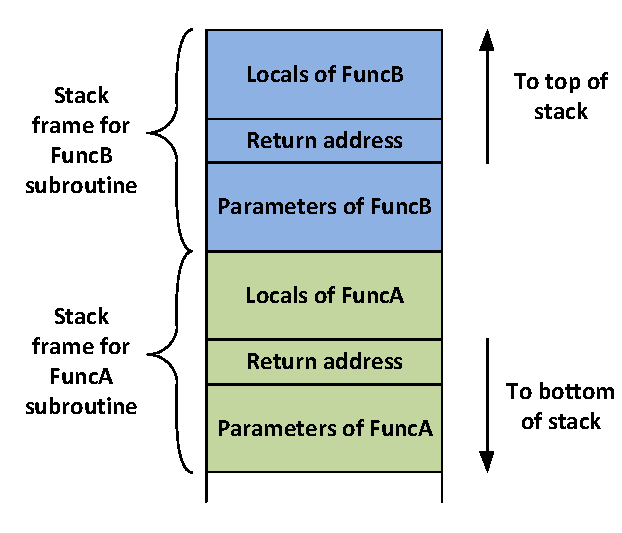
\includegraphics[height=8cm]{Figures/CallStack.pdf}
   \caption{An example call stack built of two stack frames where \emph{FuncA} is called first. Adapted from~\cite{callWiki}.}
   \label{fig:call}
\end{figure}






\section{Case Studies}
\subsection{Intel 8086}
\label{8086}
The Intel 8086 has support for procedure call instructions which automatically use the stack to organise data.
The assembler held in listing~\ref{lst:8086Caller.asm} and~\ref{lst:8086Callee.asm} is written for the Intel 8086 microprocessor.
This is a basic example of how stack frames are built to pass parameters to and from a subroutine.
The main program in listing~\ref{lst:8086Caller.asm} loads two immediate values into registers then begins building a stack frame by pushing them to the stack.  
The subroutine is called to act upon the arguments passed via the stack.
When control is passed back to the caller these set of instructions and the return value is extracted by using relative addressing from the BP then finally two stack pops completely destroy the stack frame.
It is also possible to destroy the stack frame by using an add instruction on the SP shrinking it by one entry for addition of two.
\newpage
\lstinputlisting[label=lst:8086Caller.asm,frame=single,caption=8086Caller.asm]{Code/8086Caller.asm}



When the subroutine, in listing~\ref{lst:8086Callee.asm}, is called the return address is pushed onto the stack.
This built-in support for the stack handles branching and next line address storage using a call function.
To start the BP is placed on the stack so the SP has restoration value.
Reducing the value of the SP allocates space for local variables.
The first argument is placed in memory as a local variable; this is unnecessary but serves as example.
The second argument is loaded into a working register.
The first local variable is added to the working register which is then placed in to the memory as the second local variable.
Finally the SP and the BP are restored and a return instruction hands control over to the caller. 
This is all part of the calling convention for subroutines using stack frames on the 8086 microprocessor~\cite{8086call}.
 
\lstinputlisting[label=lst:8086Callee.asm,frame=single,caption=8086Callee.asm]{Code/8086Callee.asm}



This code was tested upon an 8086 emulator~\cite{emu8086}.
The emulator provides a complete overview of the flow of data within the processor including the stack. 
Figure~\ref{fig:emu} shows the emulator during the execution of the subroutine just before the SP is overwritten with the BP.
Figure~\ref{fig:stack} is an abstraction of the stack with data labels corresponding to the subroutine. 

\begin{figure}[htb]
        \centering
        \begin{subfigure}[b]{0.5\textwidth}
                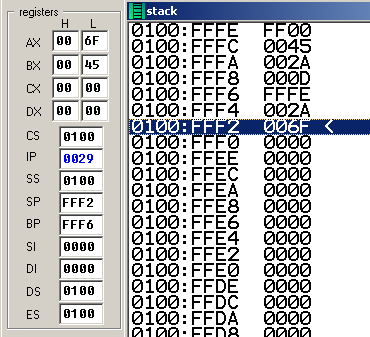
\includegraphics[height=5cm]{Figures/emu.png}
                \caption{Emulator registers and stack}
                \label{fig:emu}
        \end{subfigure}%
        \begin{subfigure}[b]{0.5\textwidth}
                \includegraphics[height=5cm]{Figures/stack.pdf}
                \caption{Stack frame configuration}
                \label{fig:stack}
        \end{subfigure}
        \caption{8086 stack operation}
        \label{fig:8086}
\end{figure}







\subsection{ARM7TDMI (using Arm Thumb)}
The ARM7TDMI is a 32-bit RISC microprocessor with an emphasis on low-power design and pipelining for high throughput which is detailed in~\cite{ARM7TDMI}.
It has two instruction sets. 
One of which is Arm Thumb, explained in~\cite{arm}, a low density compressed 16-bit subset of the ARM assembly language where the benefits are considered in~\cite{ARMs}.
It most notably assisted ARM into moving into the mobile phone market by reducing required program memory. 
A user selectable flag is set to switch between instruction sets.

This architecture does not have built-in support for calling subroutines using the stack.
When the branch instruction is used, as seen in listing~\ref{lst:ArmCaller.asm}, the program counter is overwritten with the address of the corresponding label.
The address of the next line of code, which should be returned to after the subroutine, is placed into the link register.
Calling conventions suggests leaving this register untouched and simply moving the data back into the program counter on a return.

\lstinputlisting[label=lst:ArmCaller.asm,frame=single,caption=ArmCaller.asm]{Code/ArmCaller.asm}

In this case the link register is pushed onto the stack from the subroutine therefore requiring the subroutine to pop the value into the program counter in order to return.
This is an example of important assembler context save.
If the prologue and epilogue are not respected then a call stack is never built therefore no nested functions can be used.

Listing~\ref{lst:ArmCallee.asm} holds the subroutine and handles placing the return address on the stack.
Relative addressing on the stack is required to draw the two arguments out and replace the first with the output of the function.
Although this subroutine performs the same task as code held in listing~\ref{lst:8086Callee.asm} only one local variable is used as it is never really required.
\lstinputlisting[label=lst:ArmCallee.asm,frame=single,caption=ArmCallee.asm]{Code/ArmCallee.asm}






\section{Conclusion}

It is clear that whether a microprocessor has built-in support for a stack or not the ability to call subroutines is unaffected.
The support does make calling more efficient and easier to code.

\subsection{Design Recommendation}
All instruction sets considered in this report are 16-bits in length could possibly be ported straight to the processor design.
The 8086 is a pre-RISC architecture (ref McNAlly here) that can be considered as a quite a simple CISC processor.
RISC processors are simpler to construct and rely largely   


\newpage

%TC:ignore
%References - reading referenced in text
\bibliographystyle{plain}
\bibliography{references}
\addcontentsline{toc}{section}{\protect\numberline{}References}
%Biliography - all the reading done

\makeatletter 
	\renewcommand\@biblabel[1]{\textbullet}
\makeatother

\section*{Bibliography}
\addcontentsline{toc}{section}{\protect\numberline{}Bibliography}

\begin{itemize}
   \item{
      ARM, 
      Infocenter,
      \url{http://infocenter.arm.com/help/index.jsp},
      Online. Acessed Feb 2014.\\
      - A valuable resource for all things ARM.
   }
   \item{
      Lin C.,
      Understanding the Stack,
      \url{http://www.cs.umd.edu/class/spring2003/cmsc311/Notes/Mips/stack.html},
      2004,
      University of Maryland,
      Online. Acessed Feb 2014.\\
      - General stack operation.

   }
   \item{
      Mathur S,
      \emph{Microprocessor 8086: Architecture, Programming and Interfacing},
      PHI Learning Private Limited,
      2011.\\
      - Intel 8086 microprocessor resource
   }
   \item{
      Patterson D A and Hennessy J L,
      \emph{Computer Organisation and Design: The Hardware/Software Interface},
      Morgan Kaufman,
      4th Edition,
      2009.\\
      - Lots of processor concepts and MIPS examples
   }
\end{itemize}
%TC:endignore

%\renewcommand{}{\refname}{Bibliography}
%\bibliographystyle{plain}
%
%
%\begin{thebibliography}{9}
%\bibitem{Patterson}
%  Patterson D A and Hennessy J L,
%  \emph{Computer Organisation and Design: The Hardware/Software Interface}.
%  Morgan Kaufman,
%  4th Edition,
%  2009.\\
%  - Lots of processor concepts and MIPS examples
%
%\bibitem{Mathur}
%  Mathur S,
%  \emph{Microprocessor 8086: Architecture, Programming and Interfacing}.
%  PHI Learning Private Limited,
%  2011.\\
%  - Intel 8086 microprocessor resource
%
%
%\end{thebibliography}
\end{document}
